% ==============================================================================
% LAB 119
% UNDERSÖKNING AV RC-KRETS
% ------------------------
%
% Author:
% Jonas Sjöberg     <tel12jsg@student.hig.se>
%
% License:
% Creative Commons Attribution-NonCommercial-ShareAlike 4.0 International
% See LICENSE.md for full licensing information.
% ==============================================================================

\section{Uppmätning av Bode-diagram}\label{bode}
\subsection{Beräkning}
% ------------------------------------------------------------------------------
Brytfrekvensen $f_1$ defineras som den frekvens då signalen har dämpats med
\SI{3}{\dB} och beräknas från ekv.~\eqref{eq:transfer2} enligt:

\begin{equation}\label{eq:cutoff}
  f_1 = \dfrac{1}{2 \pi R C} \si{\Hz}
\end{equation}

För kopplingen med komponentvärden enligt Figur~\ref{fig:rc-schema} beräknas
brytfrekvensen $f_1$ enligt ekv.~\eqref{eq:cutoff2}:

\begin{equation}\label{eq:cutoff2}
  \begin{split}
    f_1 &= \dfrac{1}{2 \pi \times \SI{1}{\kohm} \times \SI{100}{\nano\farad}} \si{\Hz} \\
        &= \dfrac{1}{2 \pi \times \num{1e3} \times \num{100e-6}} \si{\Hz}              \\
        &= \dfrac{10^6}{2 \pi \times 10^3 \times \num{100}} \si{\Hz}                   \\
    f_1 &= \SI{1.591549431}{\kHz}
  \end{split}
\end{equation}

Vilket ger svaret i \eqref{eq:cutoff3}; signalen dämpas med \SI{3}{\dB} vid
filtrets brytfrekvens $f_1 \approx \SI{1.592}{\kHz}$, varvid den ``rullas av''
med \SI{20}{\dB} per dekad (frekvenshöjning med en faktor av 10).

\begin{equation}\label{eq:cutoff3}
  \begin{split}
    f_1 &= \SI{1.591549431}{\kHz} \\
    f_1 &\approx \SI{1.592}{\kHz} \\
  \end{split}
\end{equation}


\subsection{Genomförande}
% ------------------------------------------------------------------------------
Genomförandet av mätningar visas i Figur~\ref{fig:bode-foto-1000},
Figur~\ref{fig:bode-foto-1300}, Figur~\ref{fig:bode-foto-1500},
Figur~\ref{fig:bode-foto-1800}, Figur~\ref{fig:bode-foto-1900} samt
Figur~\ref{fig:bode-foto-2000}.


\begin{figure}
  \centering
  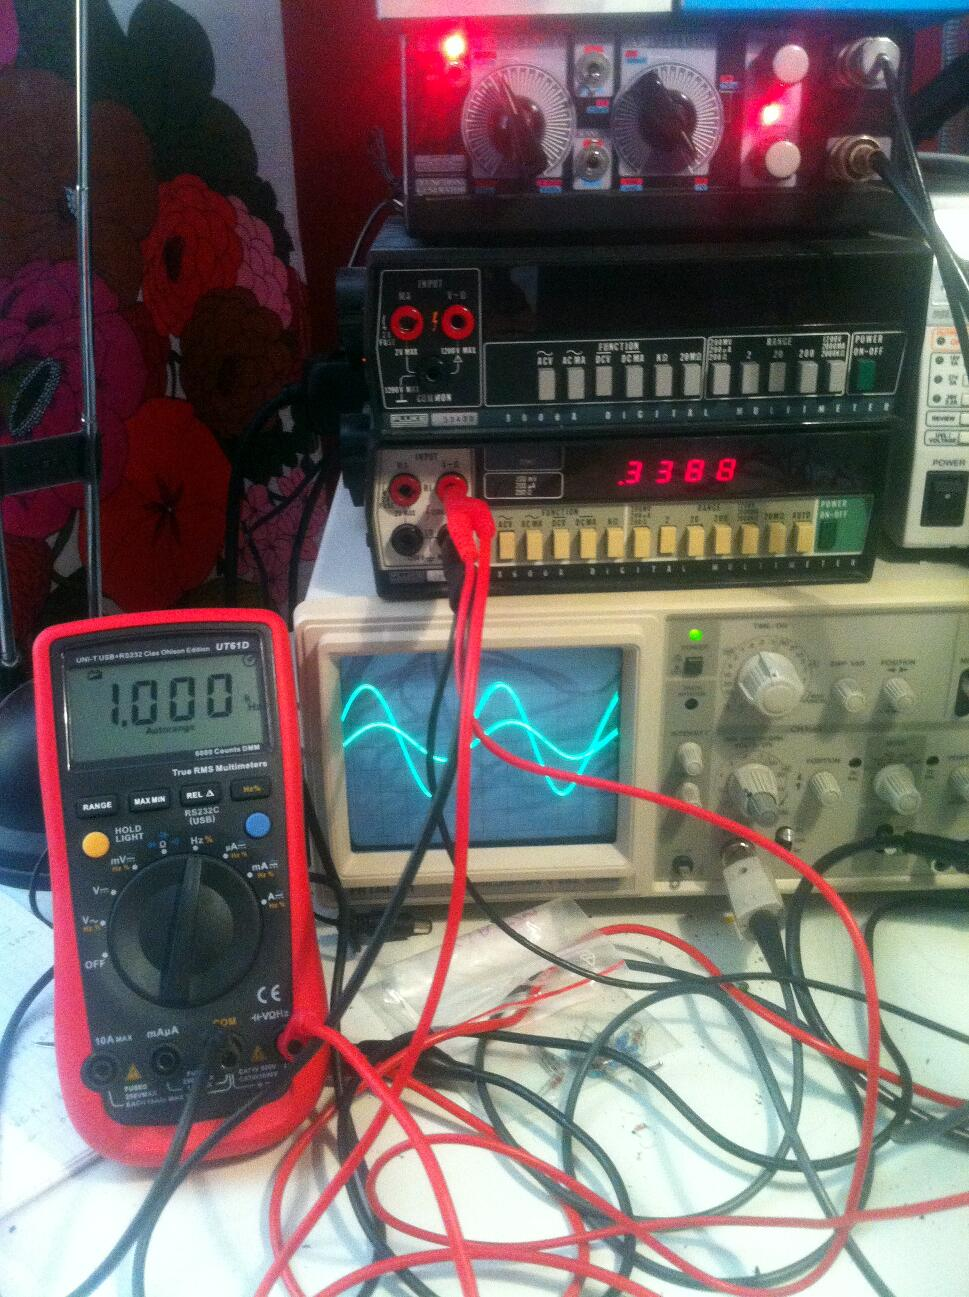
\includegraphics[width=\linewidth]{img/bode_1000Hz.jpg}
  \caption[] {Mätningar av data presenterade i Tabell~\ref{table-bode}.
              Signalfrekvens \SI{1}{\kHz}}.
  \label{fig:bode-foto-1000}
\end{figure}

\begin{figure}
  \centering
  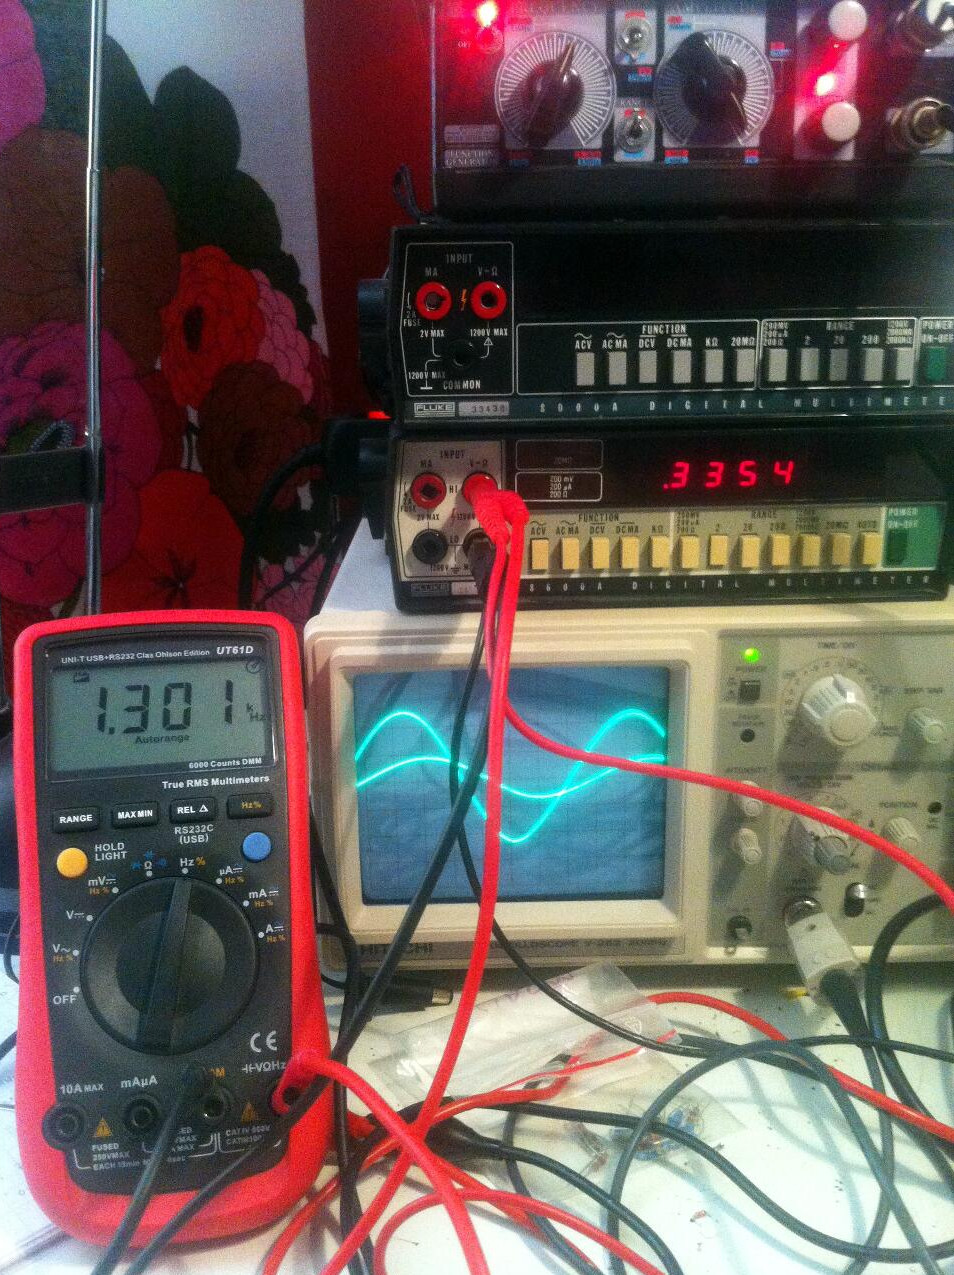
\includegraphics[width=\linewidth]{img/bode_1300Hz.jpg}
  \caption[] {Mätningar av data presenterade i Tabell~\ref{table-bode}.
              Signalfrekvens \SI{1.3}{\kHz}}.
  \label{fig:bode-foto-1300}
\end{figure}

\begin{figure}
  \centering
  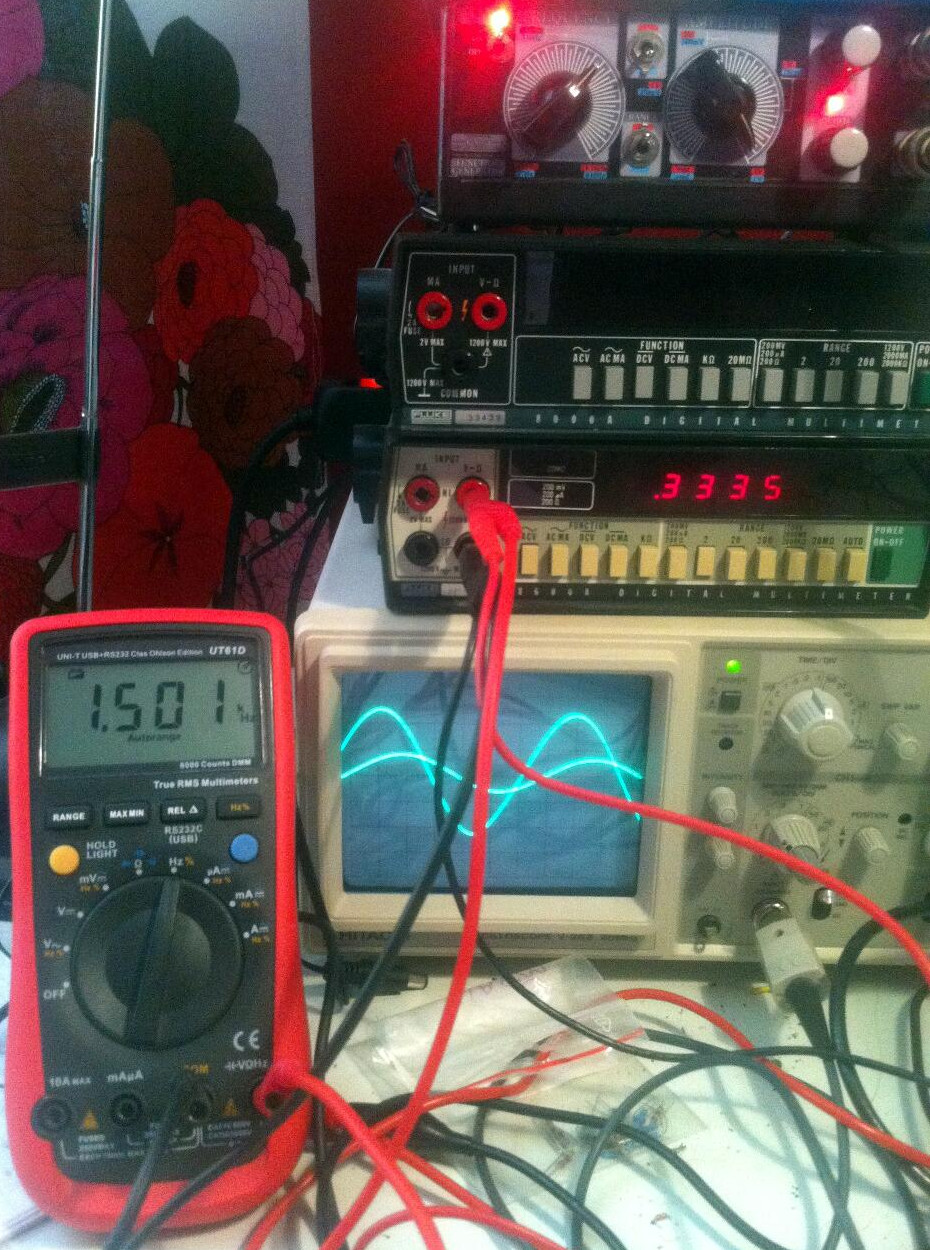
\includegraphics[width=\linewidth]{img/bode_1500Hz.jpg}
  \caption[] {Mätningar av data presenterade i Tabell~\ref{table-bode}.
              Signalfrekvens \SI{1.5}{\kHz}}.
  \label{fig:bode-foto-1500}
\end{figure}

\begin{figure}
  \centering
  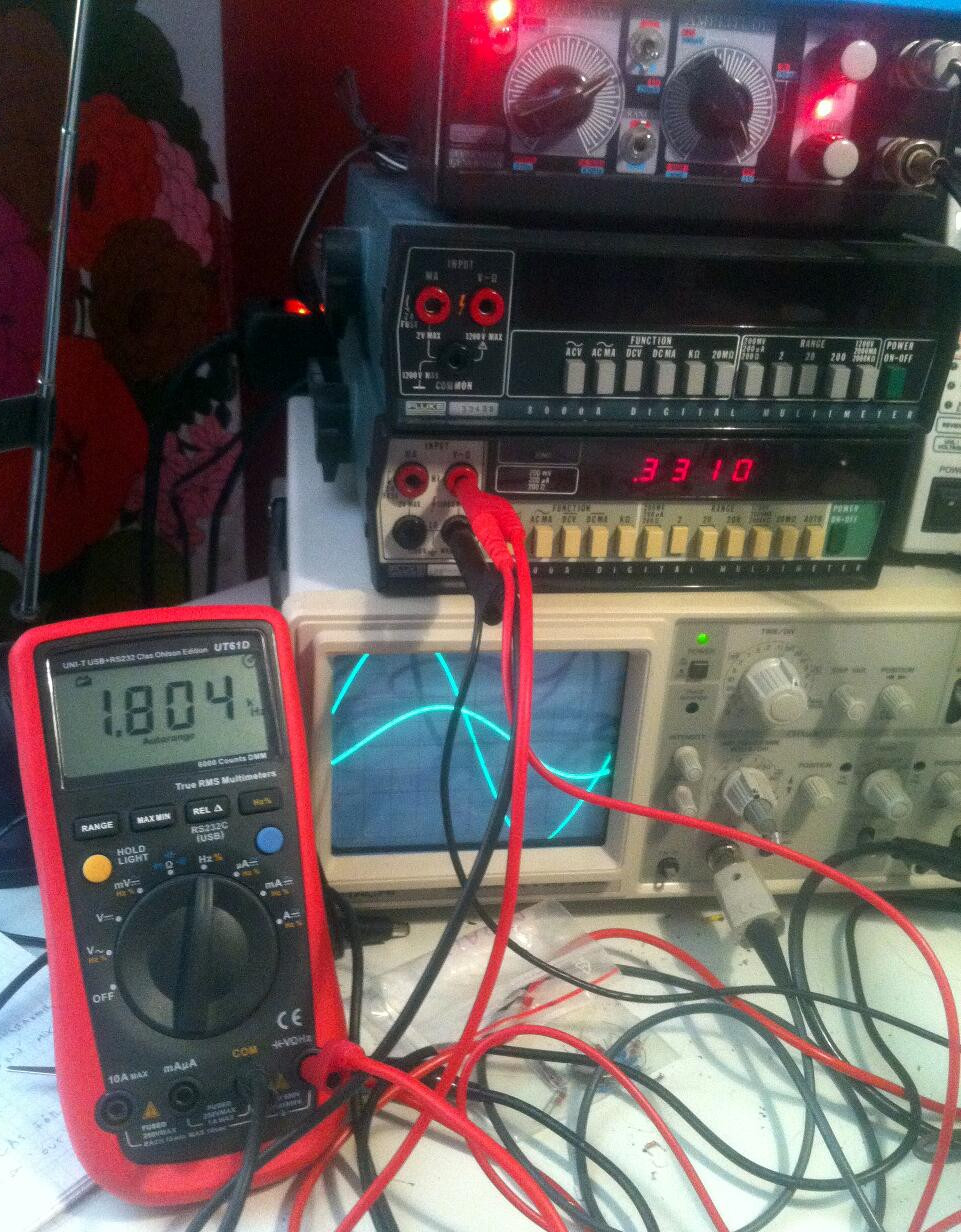
\includegraphics[width=\linewidth]{img/bode_1800Hz.jpg}
  \caption[] {Mätningar av data presenterade i Tabell~\ref{table-bode}.
              Signalfrekvens \SI{1.8}{\kHz}}.
  \label{fig:bode-foto-1800}
\end{figure}

\begin{figure}
  \centering
  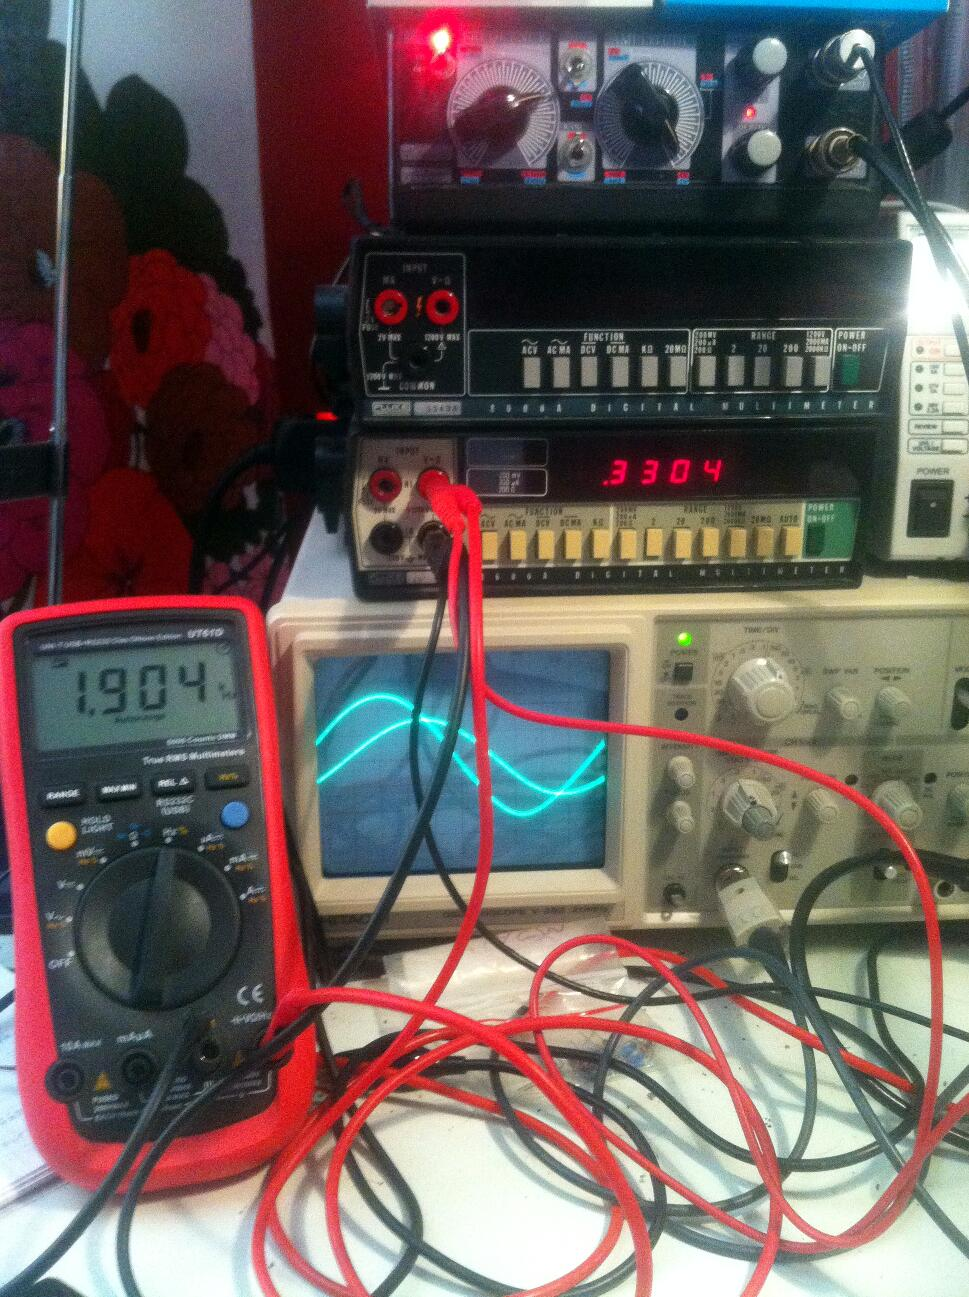
\includegraphics[width=\linewidth]{img/bode_1900Hz.jpg}
  \caption[] {Mätningar av data presenterade i Tabell~\ref{table-bode}.
              Signalfrekvens \SI{1.9}{\kHz}}.
  \label{fig:bode-foto-1900}
\end{figure}

\begin{figure}
  \centering
  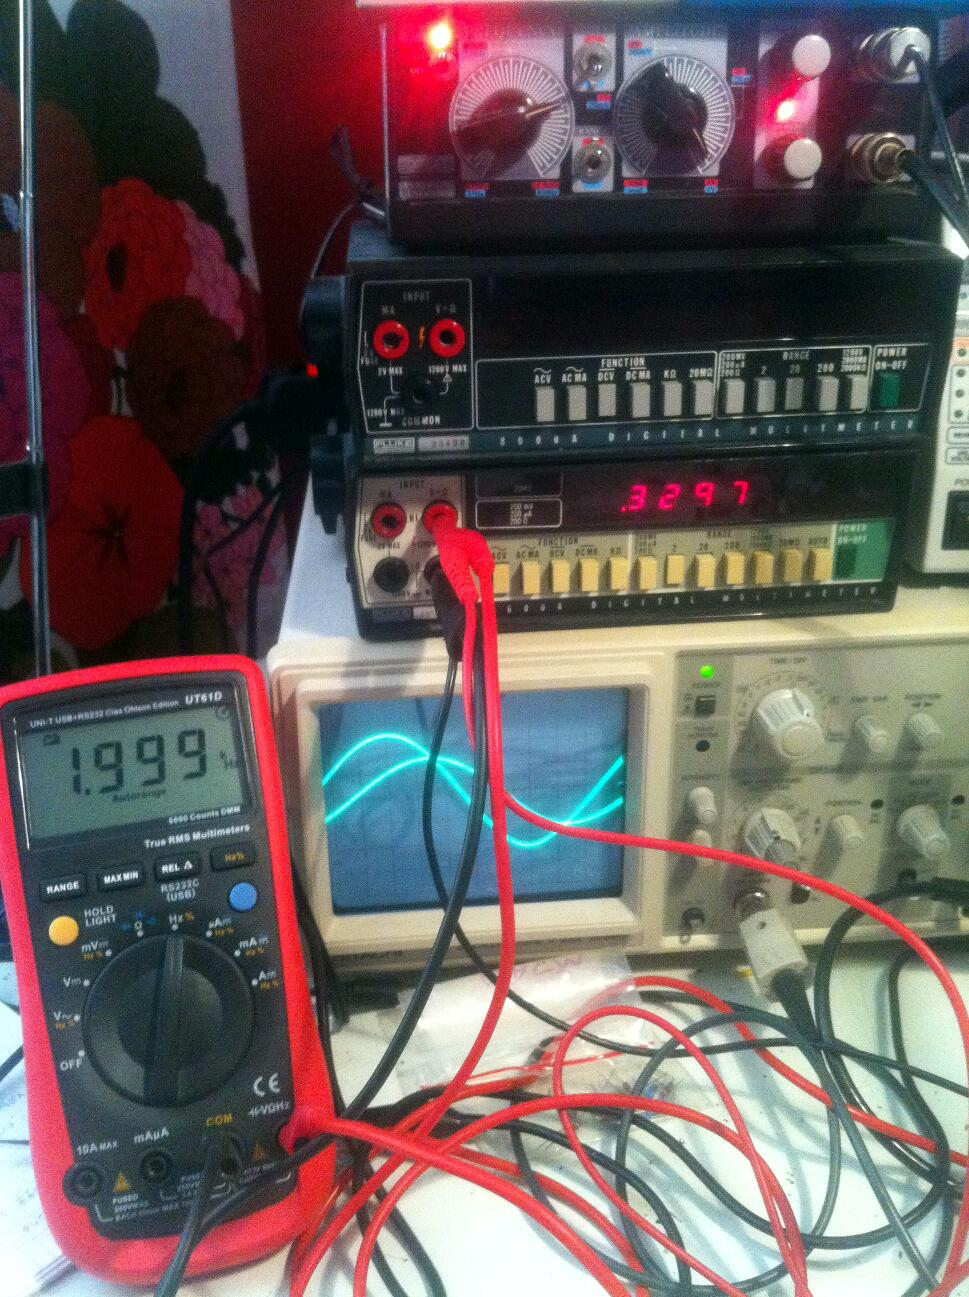
\includegraphics[width=\linewidth]{img/bode_2000Hz.jpg}
  \caption[] {Mätningar av data presenterade i Tabell~\ref{table-bode}.
              Signalfrekvens \SI{2}{\kHz}}.
  \label{fig:bode-foto-2000}
\end{figure}


\subsection{Mätresultat}
% ------------------------------------------------------------------------------
Mätresultaten presenteras i Tabell~\ref{table-bode}.

\begin{longtable}[c]{@{}ccccc@{}}
  \toprule\addlinespace
    \begin{tabular}{cc}$\text{Frekvens}        \\ (\si{\hertz})$   \end{tabular}
  & \begin{tabular}{cc}$U_{ut}                 \\ (\si{\volt})$    \end{tabular}
  & \begin{tabular}{cc}$U_{ut}/U_{in}          \\ (\si{\volt})$    \end{tabular}
  & \begin{tabular}{cc}$20 \log{U_{ut}/U_{in}} \\ (\si{\dB})$      \end{tabular}
  & \begin{tabular}{cc}$\phi                   \\ \text{(grader)}$ \end{tabular}
  \\\addlinespace
  \midrule\endhead
   100 & 1.004 & 1.004 & \SI{ 34.67}{\milli} & -3.6 \\\addlinespace
   200 & 0.998 & 0.998 & \SI{-17.38}{\milli} & -7.2 \\\addlinespace
   300 & 0.997 & 0.997 & \SI{-26.09}{\milli} & -10  \\\addlinespace % 1mS
   500 & 0.990 & 0.990 & \SI{-87.29}{\milli} & -17  \\\addlinespace % 0.1mS   ???
   700 & 0.984 & 0.984 & \SI{-140.1}{\milli} & -23  \\\addlinespace % 0.15mS  ???
  1000 & 0.958 & 0.958 & \SI{-372.7}{\milli} & -32  \\\addlinespace % 0.1mS   ???
  1200 & 0.952 & 0.952 & \SI{-427.3}{\milli} & -37  \\\addlinespace % 60uS
  1300 & 0.949 & 0.949 & \SI{-454.7}{\milli} & -39  \\\addlinespace % ????
  1500 & 0.943 & 0.943 & \SI{-509.8}{\milli} & -43  \\\addlinespace % 40uS
  1600 & 0.940 & 0.940 & \SI{-537.4}{\milli} & -45  \\\addlinespace % 35uS
  1700 & 0.938 & 0.938 & \SI{-555.9}{\milli} & -47  \\\addlinespace % ?????
  1800 & 0.936 & 0.936 & \SI{-574.5}{\milli} & -48  \\\addlinespace % 35uS
  1900 & 0.934 & 0.934 & \SI{-593.1}{\milli} & -50  \\\addlinespace % 35uS
  2000 & 0.932 & 0.932 & \SI{-611.7}{\milli} & -51  \\\addlinespace % ????
  \bottomrule
  \addlinespace
  \caption[]{Mätresultat för kretsen i Figur~\ref{fig:rc-schema}.}
  \label{table-bode}
\end{longtable}


% TODO: Bode-diagram för frekvensgång.

% TODO: Bode-diagram för Fasförskjutning.


\subsection{Simulering}
% ------------------------------------------------------------------------------
För verifiering och visualisering av den teoretiska beräkningen körs en
\texttt{SPICE}-simulering av kretsen i det GPL-licensierade open source
programmet \texttt{Qucs}\footnote{\url{http://qucs.sourceforge.net/}}.
Simuleringsuppställningen och resultatet återfinns i
Figurer~\ref{fig:bode-sim-ac}, Figur~\ref{fig:bode-sim-tran} och
Figur~\ref{fig:bode-sim-param}.

\begin{figure}\label{fig:bode-sim-ac}
  \centering
  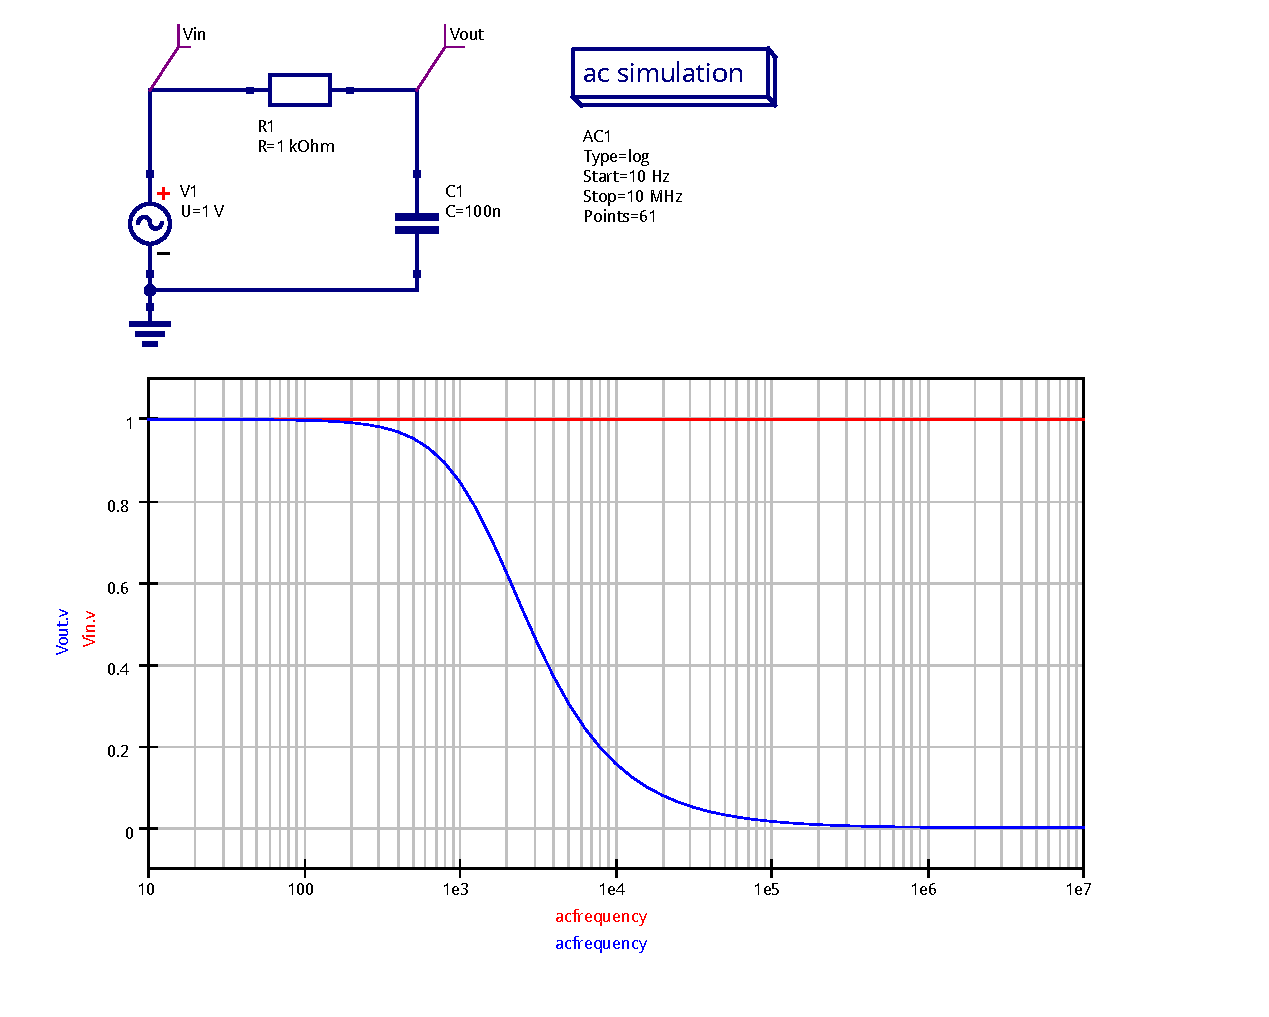
\includegraphics[width=\linewidth]{sim/ee466_lab-4_prj/uppgift-1_ac}
  \caption[] {Simulering av kretsens frekvensåtergivning.}
\end{figure}

\begin{figure}[ht]\label{fig:bode-sim-tran}
  \centering
  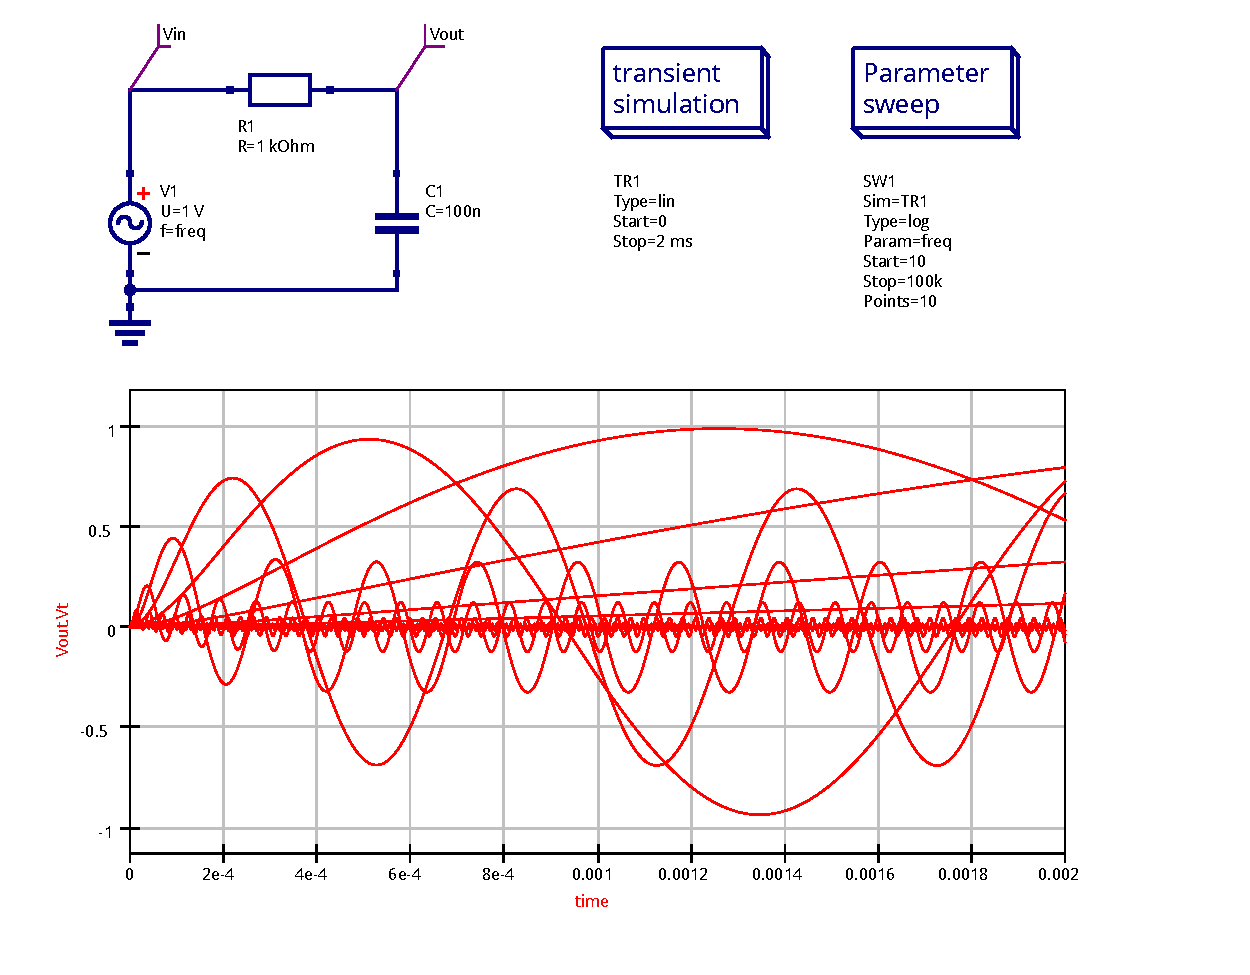
\includegraphics[width=\linewidth]{sim/ee466_lab-4_prj/uppgift-1_tran}
  \caption[] {Simulering av kretsen i tidsdomänen för olika frekvenser av $V_1$.}
\end{figure}

\begin{figure}[ht]\label{fig:bode-sim-param}
  \centering
  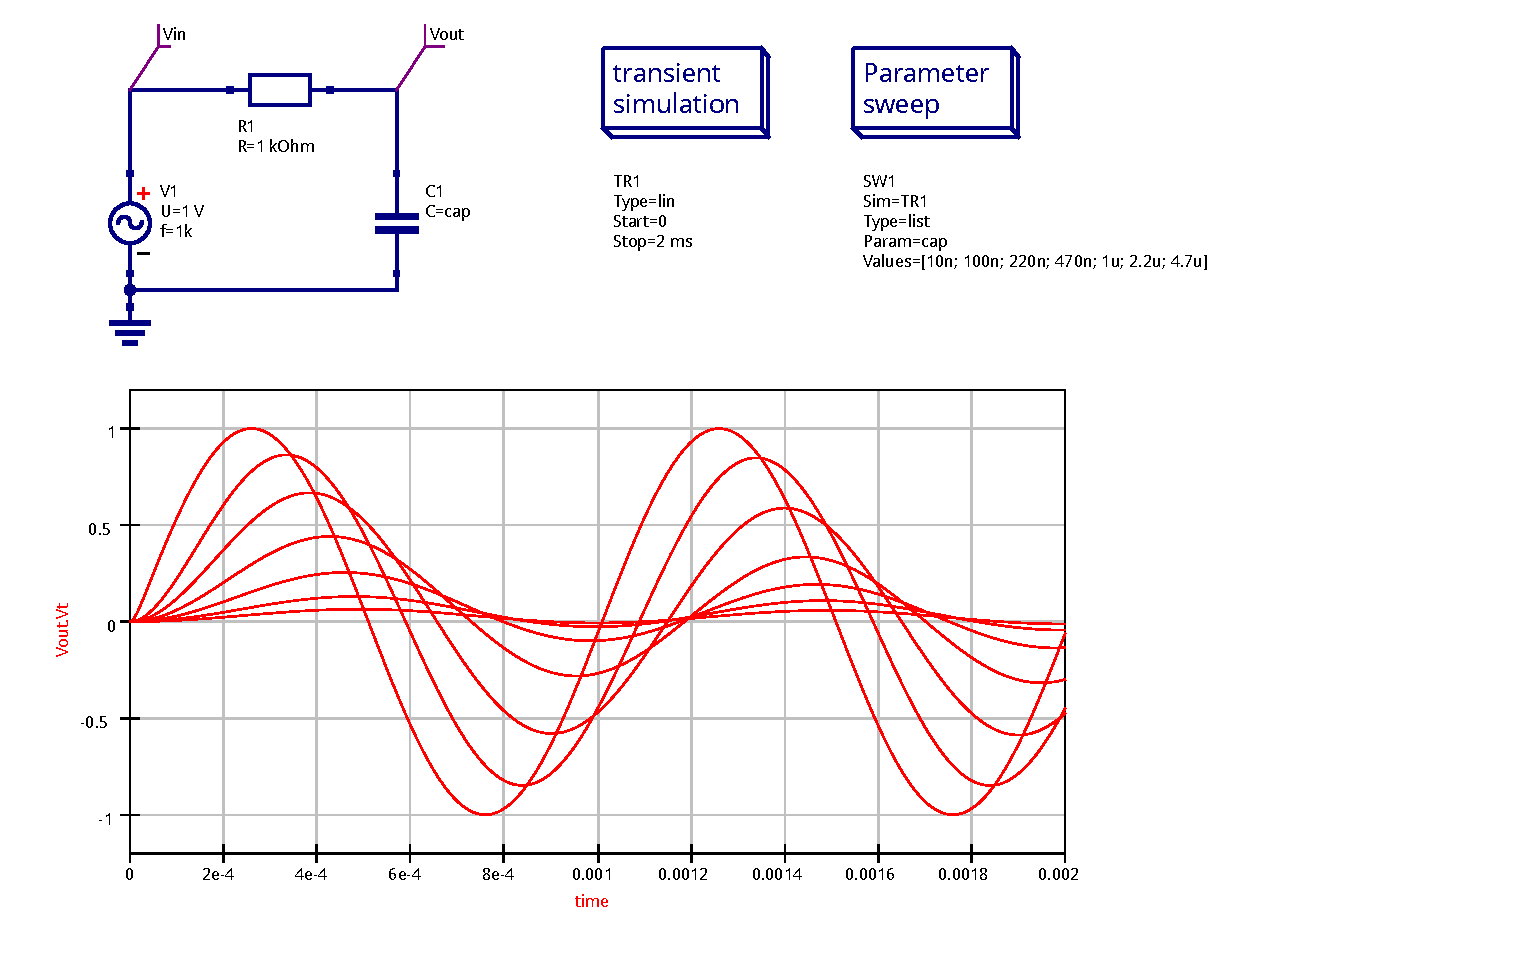
\includegraphics[width=\linewidth]{sim/ee466_lab-4_prj/uppgift-1_param}
  \caption[] {Simulering av kretsen i tidsdomänen för olika värden av $C_1$.}
\end{figure}


\subsection{Kommentar}\label{}
% ------------------------------------------------------------------------------
Mätresultaten ligger inom vad som kan antas vara rimligt för den använda
experimentuppställningen, komponenttoleranserna och mätutrustningens precision.
Den största förändringen sker inom ett begränsat frekvensområde vid och efter
brytfrekvensen. Med ett automatiserat test, med hjälp av programvara som t.ex.
\texttt{Labview} är det mer praktiskt genomförbart att göra utföra mätningar
med större precision och ett mycket större antal mätpunkter.

